%% Last update: Oct. 21, 2020
\newcommand{\ignore}[1]{}

%\subsubsection{\stid{3.07} Factorization Based Sparse Solvers and Preconditioners for Exascale} \label{subsubsect:strumpack}
\subsubsection{\stid{3.07} STRUMPACK-SuperLU} \label{subsubsect:strumpack}

\paragraph{Overview} 
% \textit{Provide an overview of your project.  You might find that the introductory text from your Fall 2017 Project Summary \url{https://confluence.exascaleproject.org/display/1ST/Fall+2017+ECP+ST+Project+Summaries} useful as a starting draft.}
This project will deliver factorization-based sparse solvers
encompassing the two widely used algorithm variants: supernodal
(SuperLU: \url{https://portal.nersc.gov/project/sparse/superlu})
and multifrontal (STRUMPACK: \url{http://portal.nersc.gov/project/sparse/strumpacK}).
STRUMPACK is
further enhanced with scalable preconditioning using
hierarchical matrix algebra. Both libraries are purely algebraic,
applicable to many application domains. We will address
several Exascale challenges, with the following
focus areas: 
(1) Develop novel approximation algorithms that have lower
arithmetic and communication complexity with respect to the size of the
input matrix;
(2) Develop new parallelization strategies that reduce
inter-process communication and expose task parallelism and vectorization
for irregular computations involving sparse data structures to better
use on-node resources;
(3) Integrate our software into higher-level
algebraic solvers such as hypre, PETSc, Trilinos, and collaborate with
ECP teams for application-specific and hardware-specific tuning
of the parameters space to achieve optimal efficiency.

Our solver technology is essential for ECP, because many 
% DOE simulation and data analysis 
codes expected to run on Exascale machines need
solutions of sparse algebraic systems, and many high-fidelity simulations
involve large-scale multiphysics and multiscale modeling problems that
generate highly ill-conditioned and indefinite algebraic equations,
for which pure iterative methods 
% such as Krylov and multigrid, albeit readily parallelizable on large machines, 
cannot converge to the solution.
The factorization-based algorithms being developed herein
represent an important class of methods that are indispensable building
blocks for solving those numerically challenging problems. Our software
can often be used as a reliable standalone solver, or as a preconditioner
for Krylov methods, or as a coarse grid solver in multigrid
methods. %, just to name a few.

\vspace{-10pt}
\paragraph{Key Challenges}
%\textit{Describe what is hard to do, why it is challenging.}
At Exascale we need to address several major challenges:
decreasing amount of memory per core, increasing impact of communication
cost and load imbalance, and increasing architectural heterogeneity.
Our new design of algorithms and codes must focus on
reducing communication and synchronization and task scheduling 
instead of floating point operation throughput. In sparse factorization
methods, we expect new bottlenecks in parts of the code
that previously received little attention. For example, the preprocessing
step involves numerical pivoting for selecting stable pivots and
symbolic factorization, which do not yet parallelize well on manycore
architectures with fine-grained parallelism.
At Exascale, direct solvers are more likely to
be used in a preconditioning strategy, for example, in block Jacobi
preconditioning, in domain decomposition methods or as coarse-grid
solvers in algebraic multigrid, which requires repeated triangular
solves. The challenge here is to mitigate the low arithmetic intensity
and high degree of data dependency.

Compared to iterative methods, the primary bottleneck of direct solvers
is the asymptotically higher growth in memory need and floating point
operations, especially for problems from three-dimensional geometry.
It is imperative to develop new factorization methods that require
much less memory and data movement.

\vspace{-10pt}
\paragraph{Solution Strategy}
%\textit{Describe your basic strategy for addressing the challenges.}
We will address these challenges in several thrust areas.
The new techniques will be implemented in the two software packages SuperLU
and STRUMPACK. The former is a widely used sparse direct solver based on
supernodal factorization and the latter is a newer direct
solver/preconditioner package based on multifrontal factorization 
and hierarchical low-rank matrix structures.
% Parallel pre-pivoting for both packages.

The improvements for SuperLU will be mainly in two areas: (1) develop
the communication-avoiding 3D factorization and triangular solve
algorithms and codes that have provably lower communication complexity;
(2) develop a synchronization-avoiding triangular solve code to enable more
overlap of communications of different processes at different substitution steps;
(3) develop new multi-GPU codes for both symbolic preprocessing step and
numerical factorization and solve steps.

In addition to exploiting structural sparsity as SuperLU does, STRUMPACK
also exploits data sparseness in the dense blocks of sparse factors using
low-rank representations, which leads to linear scaling $O(n)$ or $O(n \log n)$
memory and arithmetic complexity for PDEs with smooth kernels.
The developments for STRUMPACK will focus on several areas:
(1) develop robust stopping criteria --- both absolute and relative --- for
    adaptive (incremental) randomized sampling schemes to reveal numerical
    ranks in the low-rank compression routine. The goal is to use
    enough samples for stability, but not too many for efficiency;
(2) add OpenMP support for both HSS compression and ULV factorization routines,
    especially use OpenMP task construct to support irregular parallelism;
(3) reduce MPI communication in all stages of the code, including HSS
    construction, ULV factorization and triangular solve;
(4) in addition to HSS, develop codes to support other simpler low-rank
    formats, such as HOLDR and BLR. The HSS format has asymptotically
    lower complexity than HOLDR and BLR, but has a larger prefactor constant.
    We expect HSS to be more useful for large-scale problems while HOLDR
    and BLR are more useful for mid-range problems;
(5) work with ECP application teams to examine their specific problem
    characteristics and develop the best clustering/ordering methods to 
    reveal low-rank structures.
    
\vspace{-10pt}
\paragraph{Recent Progress}
%\textit{Describe what you have done recently.  It would be good to have some kind of figure or diagram in this section.}
\ignore{ %%%% replace the following by the new activities
In the past six months, we added more support for GPUs and
improved on-node threading performance.  To this end, we participated
in the 3.5-day ECP OpenMP Hackathon at NERSC in August 2019,
working closely with the HPCToolkit and SOLLVE teams,
as well as the OpenMP/vectorization experts from Intel.  
Using HPCToolkit revealed several performance bottlenecks.  We rewrote
the code to remove a few inefficiencies, and identified solution strategies
for the other bottlenecks.

We also worked with two ECP applications: MFEM electromagnetic diffusion
problems governed by high frequency indefinite Maxwell equations
(CEED Co-Design Center) and ExaSGD Miniapp2 -- sparse ACOPF matrices:
\url{https://github.com/LLNL/hiop/tree/sandbox/matrices/data/acopf_matrices}
}  %%%% ignored


We mainly focus on the multi-GPU developments. For SuperLU, the developments on parallel symbolic
factorization and triangular solve with one-sided communication using NVSHMEM. All the experiments
are performed on Summit.
% The main algorithmic challenges we have to overcome are: parallel tasks are of non-uniform size,
% load imbalance, and memory and communication bound operations.

For STRUMPACK we improved the GPU off-loading code. We ported the
preconditioner based on block low-rank compression to distributed
memory systems. We developed an interface from Trilinos to STRUMPACK.

We also worked with the ECP application ExaSGD team, applying our sparse solvers to
the linear systems coming from AC optimal power flow problems. The linear systems
arising from the Interior Point optimization loops are highly ill-conditioned,
and zero-pivots are encountered during numerical factorization.
We improved both STRUMPACK and SuperLU to deal with the situation and allow the factorization
to succeed and recover the solution accuracy by iterative refinement.

The other algorithmic changes and the results are detailed below.

\vspace{-5pt}
\paragraph\
\underline{STRUMPACK}  % {\bf (Pieter -- update the following)}
\begin{itemize}
\item We added GPU kernels for the extend-add (gather-scatter)
  operation used in the sparse solver, so that the entire
  factorization (or a subset fitting in device memory) can be
  off-loaded without requiring excessive amounts of data movement
  between host and device. On a single summit node, the new GPU code
  is up to 8x faster than the old algorithm.
\item STRUMPACK now supports AMD GPUs through HIP, and the hipBLAS and
  rocSOLVER libraries.
\item We added a distributed memory block low-rank preconditioner to
  the sparse solver. For a medium sized 3D $175^3$ high frequency
  Helmholtz problem, the new preconditioner is 3.7x faster than the
  sparse direct solver, and 2x faster than our previous state of the
  art preconditioner based on Butterfly compression.
\end{itemize}

\underline{SuperLU}
\begin{itemize}
\item Finished the first version of the multi-GPU path-based traversal algorithm for
  parallel symbolic factorization, including supernode detection algorithm. The new code
  showed strong scaling up to 31x speedup on 44 Summit GPU nodes.
\item Implemented the single precision LU factorization with double precision iterative refinement.
  Initial tests show up to 50-60\% speedup on 1 node Summit using 6 CPU cores and 6 GPUs.
%  The speedup mainly comes from reduced data transfer / communication.  
\item Improved the user interface for the 3D code base: developed the new redistribution routine,
  so that the users do not need to worry about setting up proper submatrices on the 2D layer
  of the 3D process grid.
\end{itemize}

\vspace{-.13in}
\begin{figure}[htb]
%\begin{minipage}[t]{0.48\columnwidth}
%% \centering
%% \includegraphics[scale=0.7]{projects/2.3.3-MathLibs/2.3.3.07-STRUMPACK-SuperLU/strumpack-Summit.pdf}
%% \caption{STRUMPACK factorization on Summit GPU.}
%% \label{fig:strumpack-parmetis-scaling}
%% \end{minipage}
%% \hfill
%% \begin{minipage}[t]{0.48\columnwidth}
\centering
%\includegraphics[scale=0.8]{projects/2.3.3-MathLibs/2.3.3.07-STRUMPACK-SuperLU/superlu-solve-Summit.pdf}
%\caption{SuperLU solve on Summit GPU.}
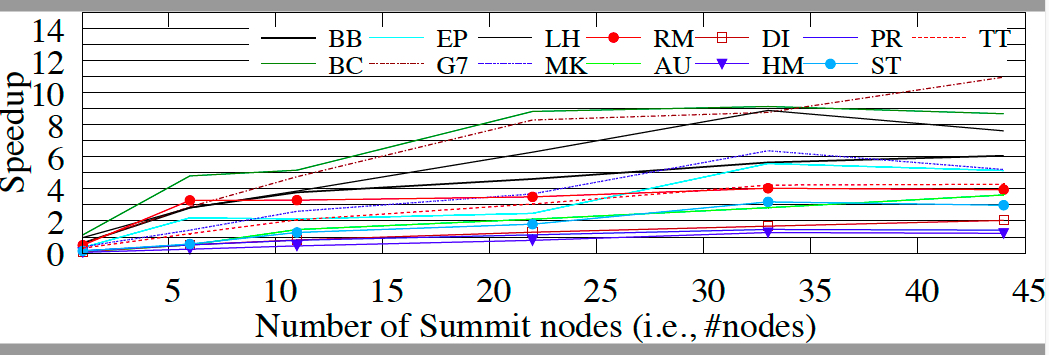
\includegraphics[scale=0.2]{projects/2.3.3-MathLibs/2.3.3.07-STRUMPACK-SuperLU/speedup_SOA.jpg}
\label{fig:strumpack-metis-scaling}
\caption{SuperLU symbolic factorization: GPU speedup over CPU, 13 matrices}
%  on Summit GPU nodes; 13 matrices}
%% \end{minipage}
\end{figure}

%%--------------------------------------

\vspace{-.135in}
\paragraph{Next Steps} Our future efforts will focus on the following areas:
%\textit{Describe what you are working on next.}
%\begin{itemize}
%\item
%%  {\bf (Pieter updates)}
 For STRUMPACK, we will work to improve the performance of the
 triangular solve on the GPU, and add GPU acceleration to the block
 low-rank solver and preconditioner.
% \item
 For SuperLU, we will work towards release of the GPU-enabled 3D code, including both numerical
 factorization and triangular solve on multi-GPUs, and release of GPU-enabled symbolic
 factorization code.
% \item 
 Furthermore, we will apply the GPTune autotuner developed from xSDK4ECP project to conduct comprehensive
 tuning in the parameter space for both STRUMPACK and SuperLU, for the ECP applications and
 on the pre-exascale machines.
% \end{itemize}

%-----------
\ignore{  %%%% from last period ....
\begin{itemize}
\item For STRUMPACK, we will improve the performance of the HSS solve
      routine, add OpenMP and reduce communication. We will implement
      the HOLDR low-rank format.
\item For both STRUMPACK and SuperLU, we will build detailed performance
      models and performance specific code optimizations for the ECP
      applications that use our solvers.
\end{itemize}
} %%%%------ ignored from last period ....

%%%%%%%%%%%%%%%%%%%%%%%%%%%%%%%%%%%%%%%%%%%%%%%%%%%%
%%%% FFTX sub-project %%%%
%%%%%%%%%%%%%%%%%%%%%%%%%%%%%%%%%%%%%%%%%%%%%%%%%%%%
\subsubsection{\stid{3.07} Sub-project: FFTX} \label{subsubsect:fftx}
\noindent

\paragraph{Overview}
The use of FFTs spans a broad range of DOE science applications, including ones represented in the exascale applications space. Most applications use the API from FFTW, an open-source library developed in the 1990's. FFTW is still used extensively on DOE HPC platforms, and the FFTW API has become the de-facto
standard FFT interface: vendors that provide FFT libraries implement
(at least a subset) of that interface. Thus, FFTW both defines the 
standard FFT library interface and is a key software component
for applications.

In the FFTX project (\url{https://github.com/spiralgen/fftx}), 
we are developing a new package for supporting FFT applications on Exascale architectures. Our approach is based on two ideas. The first is developing a backward-compatible approach that builds on the FFTW interface but extends it to enable extraction of high performance on exascale machines. The second idea is to provide a toolchain that enables the
specialization of the FFT calculation and its surrounding use case calculations (scaling, data layout transformation, marshalling/unmarshalling for communication), using code generation, symbolic analysis, automatic performance tuning, and applications-specific code generation. We will use SPIRAL, an open-source toolchain for FFT developed at CMU, as the basis for developing FFTX, and we will use specific ECP applications and target ECP exascale platforms to provide a focus for this work.

\paragraph{Key Challenges}
The traditional approach of applications using FFTs is to build up high-performance implementations out of calls to (usually 1D) FFT libraries (either FFTW or vendor libraries), interleaved with user-implemented code for use-case-specific operations. This approach may break down on the emerging ECP platforms, for two reasons. The first is that the node architectures have become more complex. Multiple cores and accelerators lead to multiple levels of parallelism, including threading and SIMD/SIMT. In addition, there are on-node complex memory hierarchies that are to varying extents user-controlled, and across which it is expensive to move data. This leads to more complex interleaving of the other components of multidimensional FFT-based applications with the core library FFTs in order to maximize the effective use of the floating point capabilities and minimize data movement across the memory hierarchy. Some of these are simply not expressible in the current FFTW interface; others can be expressed, but with great effort on the part of the applications programmer, and often with an outcome of not yielding the theoretically-predicted performance due to unexpected and opaque behavior of the FFT library software. A second problem is that the open-source FFTW libraries are no longer supported. The original developers have gone on to other things, and the support of FFTW, such as it is, is performed by volunteer labor. As a result, the extensions to support new node architectures are more brittle and provide less coverage. Expanding the feature set of FFTW to enable the more effective use of the new node architectures is not feasible, since it would entail significant modification and use of the back-end software system, which no one is supporting, and on which the expertise is no longer available.

\paragraph{Solution Strategies} 
There are three components to our approach to providing a new software stack for FFT applications.

\begin{trivlist}
\item
(1) We will design an extension of the FFTW interface that both meets the needs of the FFT use cases arising in ECP applications, and exposes the
oppportunities for obtaining high performance on current and future 
architectures. The FFTX interface will be 
backward compatible with FFTW so that legacy code using FFTW runs unmodified and gains substantially on hardware to which FFTX has been ported.
To express the additional opportunities for obtaining improved performance, we will add a small number of new features beyond the FFTW interface to express algorithmic features such as futures/delayed execution,
offloading, data placement, callback kernels, and sparsity of inputs or outputs. Such changes will have the potential to extract
much higher performance than standard FFTW calls, since higher level operations and new hardware features can be addressed. This interface will be designed as an embedded DSL, for which we will provide a standard C/C++ reference library implementation that enables rapid assessment of the interface by applications developers.
\item
(2) We will develop a new code-generation back end. FFT-based application kernels implemented using the extended FFTW interface described above will be treated as specifications. This approach allows the extraction of the algorithm semantics from source code and known library semantics, thus providing whole-kernel semantics and whole-kernel specifications. This strategy enables build-time source-to-source translation and advanced performance optimizations, such as
cross-library optimization, targeting of accelerators through off-loading, and inlining of user-provided kernels.
Our approach also allows for fine control over resource expenditure during optimization. Applications can control compile-time, initialization-time, invocation time optimization resources if needed.
\item
(3) We will develop higher-level FFT-based applications driven primarily by the requirements of ECP applications projects, with the development of interfaces between FFTX and full ECP applications part of the co-design process. The strategy of having a library implementation of the FFTX interface will enable us to use the requirements of ECP applications for the design of the expanded FFTW interface and of the SPIRAL-based toolchain; in addition, the insights provided by opening up the design / tuning space for the constituent FFTs will lead to new ways of designing the applications solvers in order to obtain high performance. We will release the resulting integrated FFT-based packages as a library, called {\em SpectralPack}.

\end{trivlist}

The core code generation, symbolic analysis, and autotuning software for this project will be based on the open-source SPIRAL software stack,
building on 20 years of research by the SPIRAL team at CMU.
SPIRAL automatically maps computational kernels across a wide range of computing platforms to highly efficient code, and proves the correctness of the synthesized code.
The SPIRAL approach has many of the same structural components as FFTW -- a high-level DSL, symbolic analysis, code generation, and autotuning. However, the approach used by SPIRAL integrates these ideas more closely into the user code, generating new source code for both the FFT calls and the glue code (e.g. pointwise operations, data motion) in an FFT-based application.


\paragraph{Recent Progress}
In the past six months, we implemented FFT use cases relevant to
 accelerator modeling and materials science using FFTX v1.0. We performed 
 initial code generation for V100 GPU-based systems and baseline performance
 measurements on Summit. We released reference implementation of FFTX v1.0
 for CPUs.

\paragraph{Next Steps} Our future efforts will focus on the following areas:
\begin{itemize}
\item Deliver high performance on a single node GPU for ECP AD use cases.
\item Use ``Plan of plans'' approach to integrate domain-specific operations
  with FFTs. 
\item Design detailed control of data placement / data motion.
\item High-level C++ API to improve productivity, broaden adoption.
\end{itemize}


